\begin{figure}[bt!]
	\begin{center}
		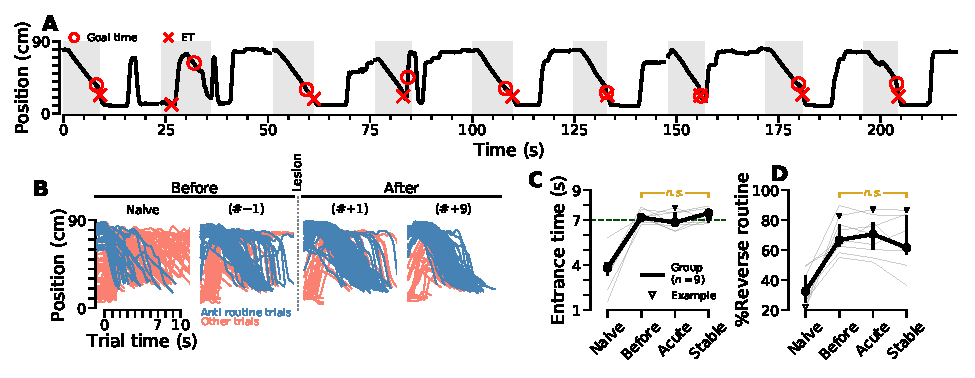
\includegraphics[width=\textwidth]{ch-lesion/figures/ReverseTreadmill.pdf}
		\caption[Preserved Motor Routine Performance After Lesion]
		{\textbf{Striatal lesion spared the performance of a motor routine.}
		\textbf{A)}
		Trajectory of a proficient animal trained in a version of the treadmill task in which the belt moved toward the reward area (rather than away from it, see \autoref{ch:methods:rev}).
		9~consecutive trials (shaded areas) and intertrials (white areas) are shown.
		\textbf{B)}
		Trajectories from a single representative animal in two sessions before and two sessions after lesion.
		\textbf{C-D)}
		Comparison of \gls{et} (\textit{C}) and percentage of the ``run-and-wait'' (reverse) routine usage (\textit{D}), before and after \gls{dls} lesion.
		}
		\label{fig:lesion:rev}
	\end{center}
\end{figure}